% Description of the project including diagrams of electrical and mechanical aspects. Depending on the complexity of the circuitry, a separate block diagram that shows functional blocks might be beneficial in addition to complete electrical schematics. The text should provide details on how the apparatus works. This section should also include a description of how your project is used.

\subsection{PWM Based Synthesis Apparatus}\label{subsec:pwm-based-synthesis-apparatus}

The actual PWM was generated on the MSP430G2553 microcontroller.
There was no need to send the signal to a DAC, as the PWM signal was directly sent to the low pass filter. 
As was discussed in Section~\ref{subsec:low-pass-filter}, the low pass filter was used to remove any unintended high frequency noise caused by the synthesizer and also to smooth out DAC volume changes. The low pass filter also allows the note OFF implementation to work: When the voltage inputted into the microprocessor was at its "default" value (both the default in the if statements in the code as well as when the voltage is at the level when no buttons are pressed), the period of the PWM was set to 2, and hence the duty cycle set to be 1. This frequency is high - 500000 Hz to be exact - and so to avoid unnecessary output interference and block short-term voltage fluctuations, this is blocked by the low pass filter. The LPF is also necessary as the MSP430 has a 32-kHz watch crystal - meaning the Nyquist frequency is 16 kHz. It may have actually been a good idea to increase the resistance such that the cutoff frequency on the LPF was below the 16 kHz mark to further avoid aliasing, but nonetheless frequencies at and above this range are still somewhat attenuated with the cutoff frequency being set to 20 kHz as we saw in Figure \ref{fig:lpfgraph}. 

This LPF was then connected to an AUX output. 
This AUX output was then connected to a speaker, however the goal of having an AUX output was to be able to connect to anything -- which is indeed the case. A speaker was used for demonstration purposes, but for measurement purposes as we see in Section \ref{sec:discussion}, this AUX output was connected to an audio interface to be able to be measured. This allowed us to analyze the signal on a computer, instead of having to use a microphone to record the signal which would lead to a less accurate representation of the signal.
The actual circuit diagram for the output is very simple (as it's just a low pass filter and a speaker), and will be included in Section~\ref{subsec:apparatus-details}.


\subsection{Apparatus Details}\label{subsec:apparatus-details}

The final rendition of this project is relatively simple in terms of electronics.
We begin by sending a signal of the same voltage to 10 different buttons, which act as the user control for the frequency of the wave emitted from the PWM\@.
The project is intended to be used similarly to a piano, with the 10 buttons available corresponding to various keys on a piano, ranging from A4 to C6, excluding sharps and flats in the note range.
When these buttons are pressed, the corresponding amplitude of the input signal is changed by sending the bits to a 10 bit DAC, which was done using a resistor ladder based on the R-2R architecture, where the resultant signal is read through a 10-bit ADC (thus allowing for the same level of precision for the DAC as is available for the ADC) that is built into the MSP430G2553 microprocessor. 
When the ADC decodes the input, the period of the PWM signal accordingly by modifying a global variable.
The duty cycle is then set to always be 50\%, by bit shifting the value of the global variable to the right by 1 bit.
Finally, the signal is outputted, and heard by the user. 

The code for this implementation is in Appendix \ref{sec:appendix-d:-pwm-synthesizer-code}, and the circuit diagram is shown in Figure \ref{fig:circuit_diagram}. It was discovered that a USB power supply to the switches was not necessary, and the whole project could be powered by connecting the ground of the MSP430 to the switches itself as we see in the diagram. While this \textit{works}, this method may also be the rationale behind the unexpected voltage fluctuation (hence frequency fluctuation) observed in the output. It would have been a smart idea to separate the grounds and power the inputs separately. 

% include circuit diagram

\begin{figure}
    \centering
    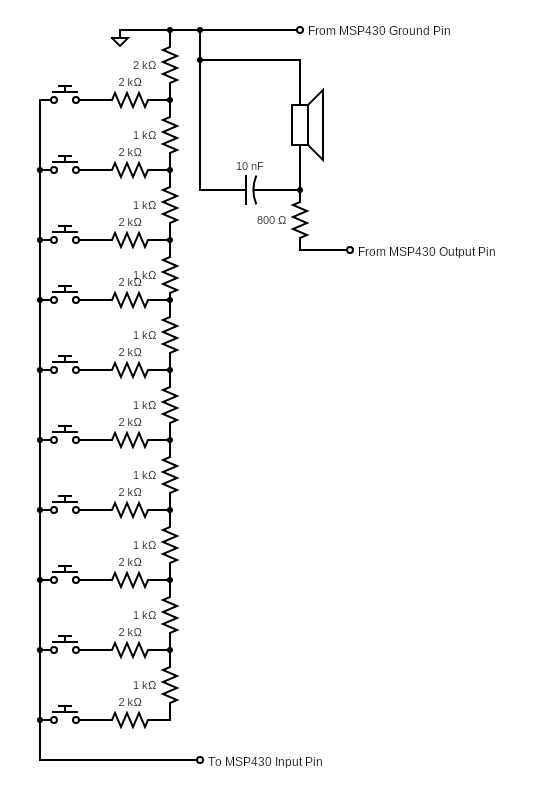
\includegraphics[width = 0.8 \textwidth]{circuit.png}
    \caption{Circuit diagram for PWM-based synthesizer. Self-powered through the MSP430. Note that the speaker is just denoting the existence of an audio output, and is actually the AUX output and not necessarily an actual speaker. }
    \label{fig:circuit_diagram}
\end{figure}






\subsection{How the project is used}\label{subsec:how-the-project-is-used}

The use of the project is relatively simple: The user plugs in the MSP430 to a power source, and plugs in headphones or a 3.5mm TRS cable to the output port. Once the synthesizer is powered on, the user plays the keys like a piano, where A4 is the leftmost key (assuming orientation of synthesizer is such that the headphone jack is facing the user, and the low pass filter is to the right of the buttons), and C6 us the uppermost key. 


\subsection{Previous Apparatus Renditions}\label{subsec:previous-apparatus-renditions}

As the initial intention of this project was to include MIDI compatibility, it is important to also include circuit diagrams for this, given it offered different methods of user interaction.
The rendition of the project that allowed for MIDI input was the 3 oscillator version (which, as will be discussed in the Results section, did not work properly due to hardware limitations).
Thus, the apparatus diagram below will reflect the legacy oscillators. The MIDI compatible circuit diagram is shown in Figure \ref{fig:3oscillatordiagram}. 

\begin{figure}
    \centering
    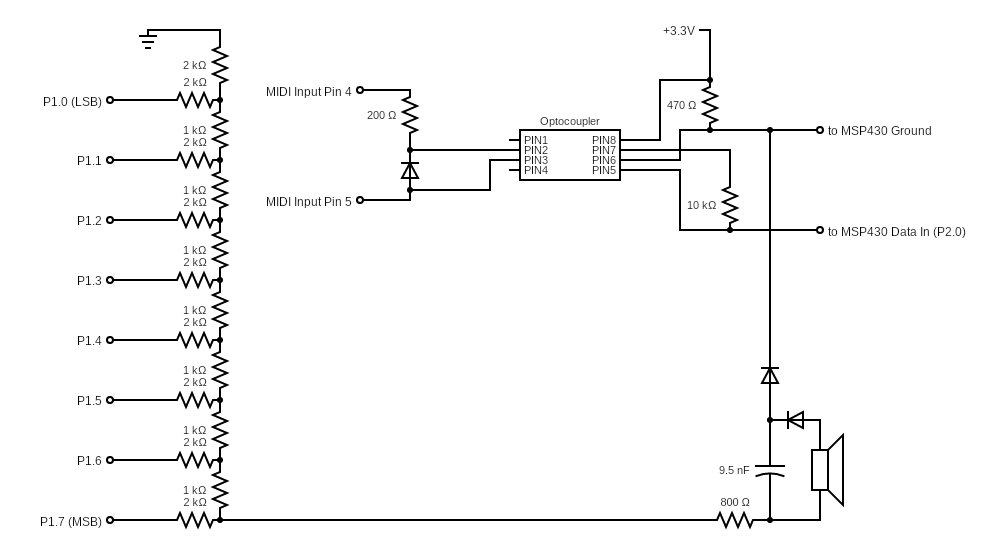
\includegraphics[width = 0.98 \textwidth]{midicircuit.png}
    \caption{Circuit diagram for the MIDI compatible, 3 oscillator version. Note that the speaker is just denoting the existence of an audio output, and is actually the AUX output and not necessarily an actual speaker.}
    \label{fig:3oscillatordiagram}
\end{figure}

Note that the sending of the output through the 8 separate pins instead of the single output pin is due to sending the direct digital signal to an 8 bit DAC, as using just a PWM does not require the use of a DAC (unlike adding the 3 waveforms together). 
Adding the 3 waveforms together would certainly be \textit{possible} using a PWM, but would be jsut as computationally expensive. 
The reason that this circuit diagram is still being shown and discussed is because it was the original intention of the project, and is significantly more complicated, thorough, and playable than the PWM version - if it worked (limitations and reasons why are discussed in Section \ref{sec:results}. 
The MIDI was being sent by an Edirol UA 25-EX Audio Interface, controlled by Presonus Studio One. 

